\subsection{Empirical Evaluation}\label{sec:eval}
\subsubsection{Comparison With Prior Work} \label{sec:eval_comp}
We compare our noisy min-hash (NMH) protocol $\PPH$ with the current
state-of-the-art approach, called sketch-flip-merge
(SFM)~\cite{ICML:HehTinCor23} and the generalized randomized response mechanism
(GRR)~\cite{sisap:AumBouSch20}. %
In particular, we evaluate the trade-off between communication cost and cardinality estimation accuracy, while achieving (almost) the same level of privacy guarantee as follows: 
\begin{itemize}
    \item For a given privacy parameter $\epsilon$ (with $\delta$ fixed to $2^{-40}$), we choose the right amount of noise for our protocol and vary the number of hash functions $k$ to measure the communication cost and estimation accuracy trade-off.
    \item We then compare these accuracy results with the state-of-the-art protocols using the same communication and privacy parameter. 
    
    We use the relative root mean squared error (RRMSE) of the union size as our accuracy metric. This choice is primarily to ensure a fair comparison between our protocol and the SFM protocol. Further details on this matter are provided in the discussion of the SFM protocol below. 

    In Figure~\ref{fig:mh_sfm_grr_acc}, we demonstrate the comparison of NMH, SFM, and GRR. 

\end{itemize}
%



\paragraph{Our protocol.}
We calculate the communication of our protocol $\PPH$ with $\F_{\psica}$ instantiated with the PSI-CA protocol described in
Figure~\ref{pro:psica}.
It is a variant of the protocol in~\cite{DGT12},
where $H_2$ is applied to $\{a'_i\}_{i \in [v]}$ and $\{b'_j\}_{j \in [w]}$ in
order to reduce the communication. 
The original protocol is secure under the DDH
assumption in the random oracle model. Essentially the same security proof found
in the original paper can be applied to show the security of this variant, when
$H_2$ is also modeled as a random oracle. 

\protocol{Private Set Intersection Cardinality}{PSI-CA Protocol.}{pro:psica}{!tbh}{
Let $G$ be a multiplicative group of order $q$. 
Let $H_1:\zo^* \to G$ and $H_2:\zo^* \to \zo^\lambda$ be hash functions. 

\textbf{Input:} $P_1$ has $C = \{c_1, \ldots, c_v\}$ and $P_2$ has $S = \{s_1, \ldots, s_w\}$.

 \begin{enumerate}
    \item $P_1$ samples a random exponent $R_c \from \ZZ_q$.  For $i \in [v]$, $P_1$ computes $a_i = H_1(c_i)^{R_c}$. $P_1$ sends $(a_1, \ldots, a_v)$. 

    \item $P_2$ samples $R_s \from \ZZ_q$  and computes 
    $(a'_1, a'_2, \ldots, a'_v) = \shuffle(a_1^{R_s}, \ldots, a_v^{R_s}).$
    $P_2$ also computes 
     $(b_1, b_2, \ldots, b_w) = \shuffle(H_1(s_1)^{R_s}, \ldots, H_1(s_w)^{R_s}).$
    $P_2$ sends $(H_2(a'_1), \ldots, H_2(a'_w))$ and $(b_1, \ldots, b_w)$ to $P_1$. 
    \item 
    $P_1$ computes $(b'_1, \ldots, b'_w) = (b_1^{R_c}, \ldots, b_w^{R_c})$. $P_1$ outputs the following value: \[| ~\{H_2(a'_1), \ldots, H_2(a'_v)\} \cap \{H_2(b'_1), \ldots, H_2(b'_w)\}|. \]
\end{enumerate}
}
We briefly sketch the security proof here while referring the full proof to the original paper~\cite{DGT12}. We first show the simulator for the corrupted $P_1$. Let $t$ be the protocol output (i.e., set intersection cardinality). The simulator chooses random $t$ indices $(i_1, \ldots, i_t)$ (resp., $(j_1, \ldots, j_t)$) from $[v]$  (resp., $[w]$).  In order to prepare $(b_1, \ldots, b_w)$, the simulator replaces $H_1(s_{j_k})^{R_s}$ (for $k \in [t]$) with $H_1(c_{i_k})^{R_s}$, and the remaining values $H_1(s_h)^{R_s}$ are simulated with random numbers. Since $H_1$ is a random oracle (i.e., for an input $x$, we have $H_1(x) = g^r$ for a random $r$), this simulation is indistinguishable under the DDH assumption. When $P_2$ is corrupted, the first message $\{a_i = H_1(c_i)^{R_c} : i \in [v]\}$ is simulated by random values. The simulation is also  indistinguishable under the DDH assumption.
The above PSI-CA protocol
exchanges $v + w$ elliptic curve points and $w$ hashes, resulting in $(v +
w)\cdot 256 + w\cdot 80$ bits. In protocol $\PPH$, the parties will run
this PSI-CA protocol by setting $v = w = k + 2\ell_B$. 


\paragraph{Sketch-Flip-Merge (SFM)~\cite{ICML:HehTinCor23}.}
%
While our main focus is on comparing the accuracy of Jaccard Index estimation,
in the absence of available code, we had to rely on their analysis of the
relative root mean squared error (RRMSE) of cardinality estimation instead of
Jaccard Index estimation. 
%
This poses challenges in evaluating the accuracy of the Jaccard Index for SFM.
In particular, although the Jaccard Index can be estimated by calculating the
ratio of estimated intersection size over the estimated union size, its RRMSE
cannot be directly calculated from RRMSEs for the intersection and union sizes.
This is because the two estimates have dependency, and we can only conjecture
that the derived estimate through the division operation will probably have a
worse RRMSE. 

In the end, giving a slight advantage to SFM, we decided to focus on the
accuracy of cardinality estimation of the size of the union only. In our case,
the union size was estimated based on the Jaccard Index from the min-hash
protocol and $n_A$ and $n_B$.
%
Following the approach of SFM~\cite{ICML:HehTinCor23}, we perform $m = 1000$
estimates to measure the accuracy in the form of relative root mean squared
error (RRMSE); that is, letting $\hat{n}_{U,1},\dots,\hat{n}_{U,m}$ be the union
size estimates, and $n_U$ be the real union size, we define
    $\text{RRMSE}(\hat{n}_{U,1},\dots,\hat{n}_{U,m}; n_U)$ to be
    $\frac{1}{n_U}\sqrt{\frac{1}{m}\sum_{i=1}^m(\hat{n}_{U,i}- n_{U})^2}$. %
To match the communication complexity, we set the sketch of SFM to be a $(B
\times P)$-bit matrix such that $B \cdot P = 592w$ and $P = 24$. 

\paragraph{Generalized Randomized Response (GRR)~\cite{sisap:AumBouSch20}.}
We also compare our protocol with the generalized randomized response MinHash
protocol in~\cite{sisap:AumBouSch20}. Following their guidance in experiments,
we select the range of their hash function to be a single bit and let their
protocol use $592w$ hash functions to match our communication
cost.

Since their actual
protocol would take too long to run for large $n$ and $k$,
in order to facilitate the large number of hash functions, we wrote code simulating 
the error based on their privacy and utility analysis. As with the other protocols, we perform 1000
estimates to lower the variance of the errors. To align with our other
comparison with SFM, we report the relative root mean squared error of the union
size. 

\medskip
\begin{minipage}[b]{0.45\textwidth}
\centering
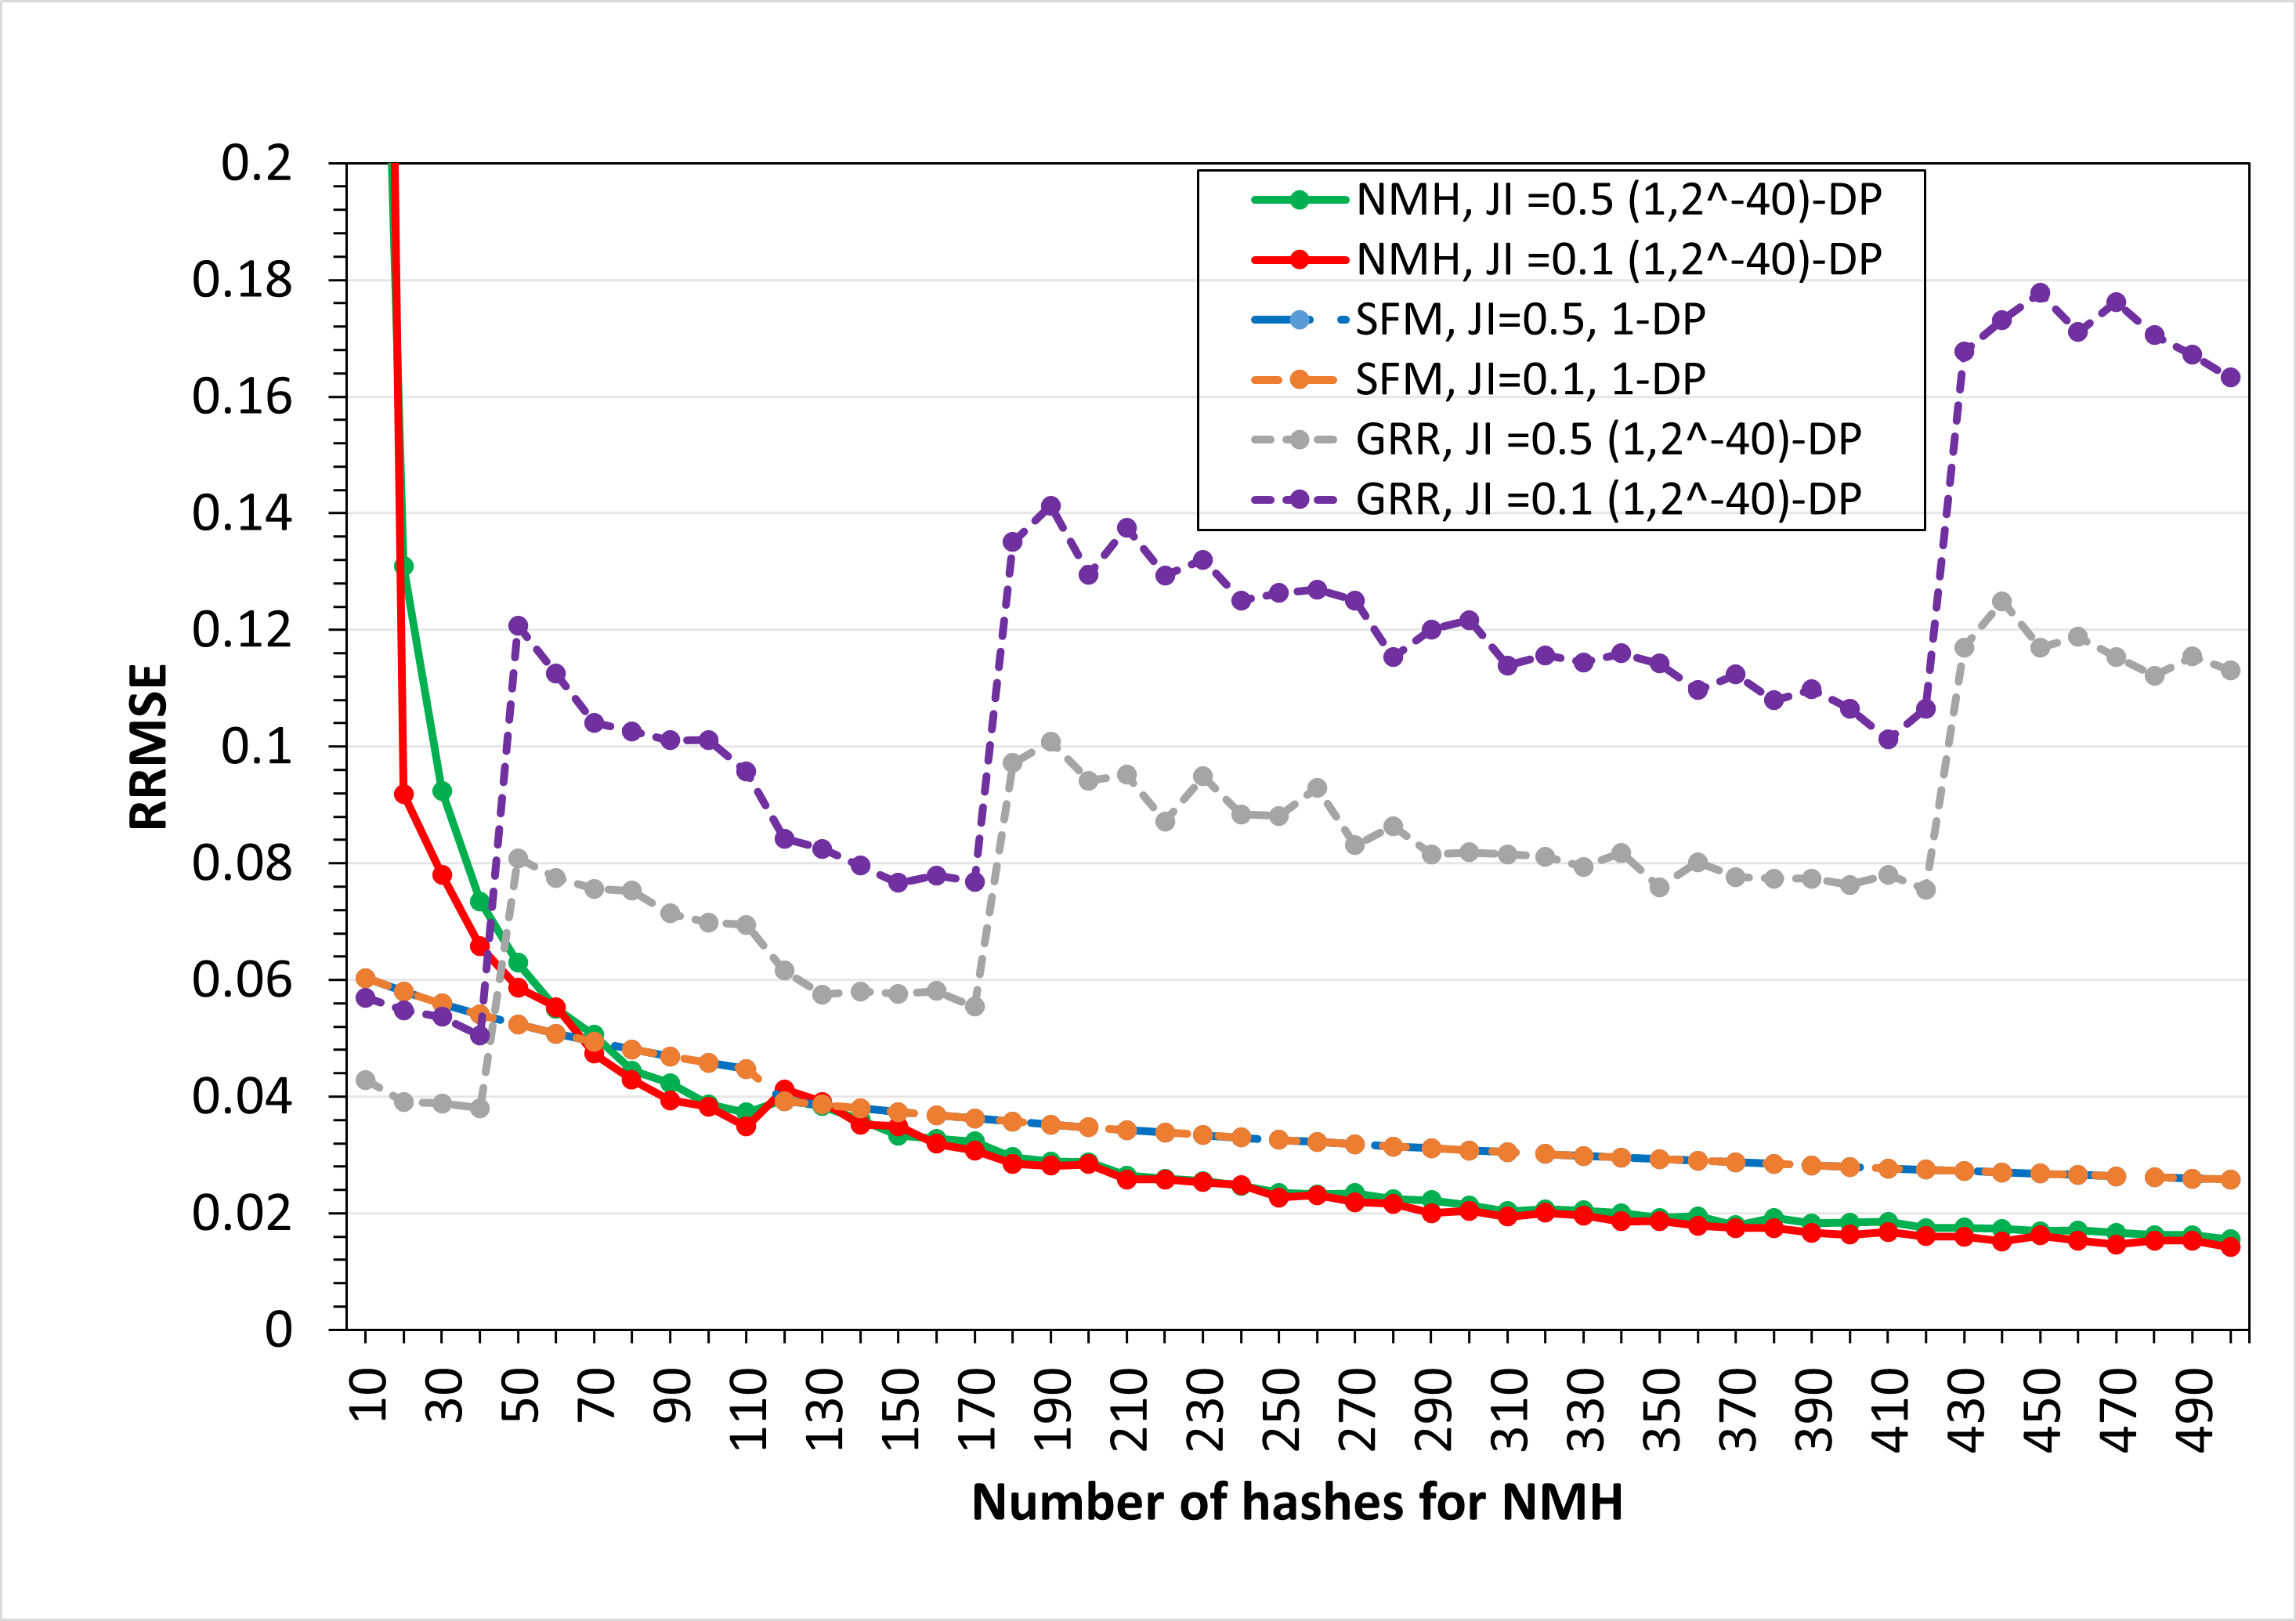
\includegraphics[width=\textwidth]{src/minhash/Images/MHL_SFM_GRR_Accuracy_1eps.png}
\captionof{figure}{Accuracy: NMH, SFM, GRR. }
\label{fig:mh_sfm_grr_acc}
\end{minipage}
~~
\begin{minipage}[b]{0.45\textwidth}
\centering
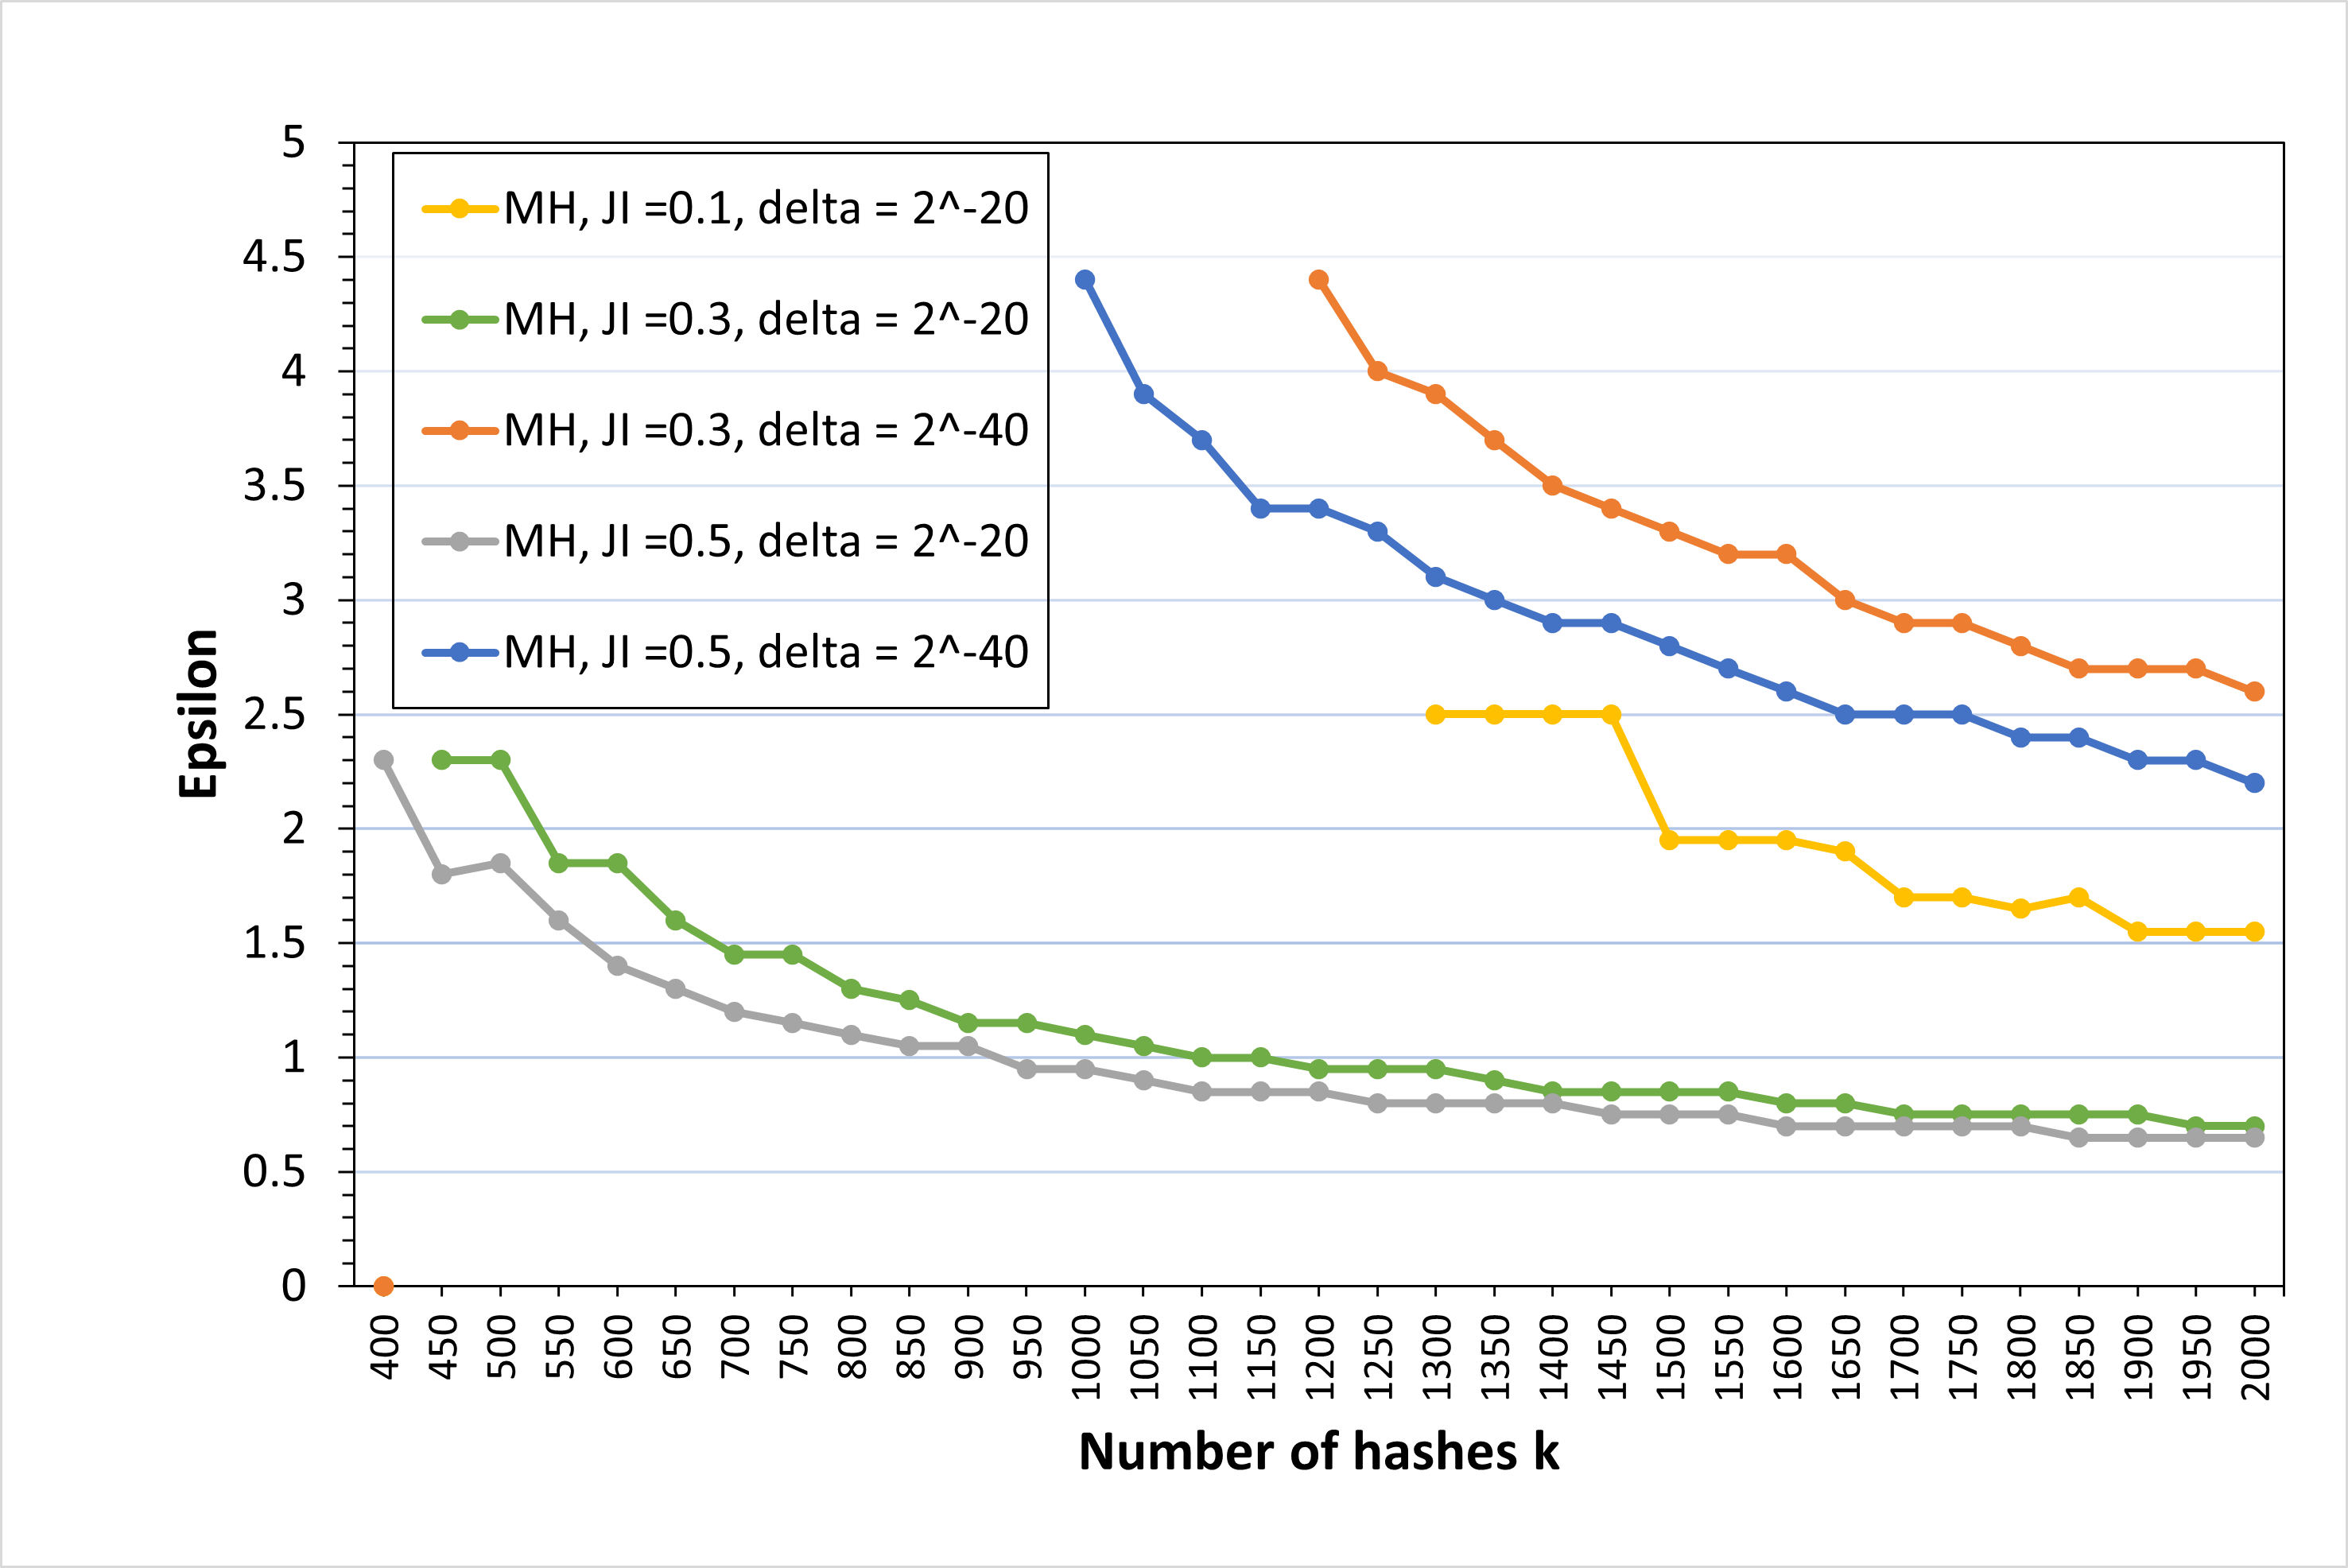
\includegraphics[width=\textwidth]{src/minhash/Images/MH_k_vs_eps_1mil.png}
% \vspace{-1em}
\captionof{figure}{DDP based on $k$, and $JI$} 
\label{fig:mh_k_vs_eps}
\end{minipage}

\paragraph{Comparison Results.} 
In Figure~\ref{fig:mh_sfm_grr_acc}, we demonstrate the comparison of NMH, SFM, and GRR. We set $n = 10^6$. The result shows that our error
is consistently smaller than both SFM and GRR for a reasonable range of
communication costs, which corresponds to the usage of $k \in [100, 500]$ hashes for our noisy min-hash protocol. 
Specifically, as we increase the number of hash functions, both our protocol and SFM achieve increased accuracy, due to larger sketch sizes that better represent the input sets. On the other hand, while GRR performs well with smaller communication, adding more communication becomes counter productive. This is because each additional bit in their protocol corresponds to an extra hash function output, which increases the noise needed to achieve the same privacy guarantee. Finally, both GRR and our protocol exhibit spikes in the accuracy trends, corresponding to crossover points where a significant amount of additional noise is required to keep $\delta$ from getting above $2^{-40}$. 

In concluding remarks, it is noteworthy that both SFM and GRR protocol discloses
the entire noisy sketch, revealing collective information about the party's
input set. We note that differential privacy does not prohibit revealing
collective information about the inputs; rather, it mandates that individual
contributions should not be discernible in the output. In contrast, our min-hash
protocol employs secure two-party computation and discloses no information about
the input set, except for the final $(\lg k)$-bit output.
%
% \footnote{The minimal
% amount of leakage in the protocol is actually crucial to maintain high min-entropy in the
% honest input during future min-hash protocol executions.}
%
When deciding which scheme to use, depending on the specific use case, this
observation may need to be taken into account.

\subsubsection{DDP of Noiseless Protocol}
We empirically evaluate the DDP guarantee
for the noiseless min-hash protocol in the public hash setting, in which each element in the secret set has high entropy. 
As before we set $n_A = n_B = 10^6$. 
%
Figure~\ref{fig:mh_k_vs_eps} shows how the privacy parameter $\ee$ changes with the number $k$ of iterations. Although we demonstrate the results for $JI \leq 0.5$,  the results for $JI > 0.5$ are similar. We omit the data points where $\epsilon$ is greater than 5, which happens when $k$ is small, and focus on the more meaningful $\epsilon$ range. 
We observe the following:


\begin{itemize}
\item 
Roughly speaking, when the number $k$ of iterations of the min-hash protocol is
reasonably large (at least 500), the noiseless min-hash protocol provides a
decent level of DDP with privacy parameter $\ee \in [0.5, 5]$. 

\item 
Higher values of $k$ correspond to improved privacy parameters.  Note that as
$k$ grows, more iterations will be $\theta$-good. Since hashes of
non-intersecting items work as noise in $\theta$-good iterations, more
$\theta$-good iterations will essentially amount to adding more noise, therefore
offering better privacy guarantee.

\item 
When $k$ is the same, the best privacy parameter is achieved when $JI$ is around $0.5$. 
This is due to the likelihood that a hash function is $\theta$-good being maximized when striking a balance between the two conditions stipulated in Definition~\ref{def:theta-good}: (i) the hash of an intersecting item should be the minimum hash value, and (ii) the minimum hash value is neither too large nor too small. 
\end{itemize}



% \subsection{Empirical Evaluation (Old)}\label{sec:eval}
% We conduct empirical evaluations in the public min-hash setting with high individual min-entropy to determine the proper parameter ranges for privacy.

% Let $k$ denote the number iterations used in the min-hash (MH) protocol, $JI$ be the Jaccard Index, and $(\ee, \dd)$ be the privacy parameters.  Throughout the experiments, we use $n_A = n_B = 10^6$.  

% \paragraph{Relations between $(\ee, \dd)$, $JI$ and $k$.} 
% In Fig.~\ref{fig:1mil_e_d_J_K_public}, the left graph shows how the privacy parameters change with respect to $JI$ when $k = 2000$. 
% %
% The right graph in Fig.~\ref{fig:1mil_e_d_J_K_public} illustrates the
% variations in $k$ relative to $JI$ across different privacy parameter settings.
% These graphs highlight the following observations:

% \begin{itemize}
%  \item 
% Keeping $k$ fixed, the privacy parameters become optimal when $JI$ is around $0.5$. 
%  \item 
% Keeping $(\ee, \dd)$ fixed, the protocol requires the minimum $k$ when $JI$ is around $0.5$. 
%  \item 
% Keeping $JI$ fixed, higher values of $k$ correspond to improved privacy parameters.  
% \end{itemize}
% The first two observations are due to the likelihood that a hash function is $\theta$-good being maximized when striking a balance between the two conditions stipulated in Definition~\ref{def:theta-good}: (i) the hash of an intersecting item should be the minimum hash value, and (ii) the minimum hash value is neither too large nor too small. For the last observation, note that as the number $k$ of total iterations grows, more iterations will be $\theta$-good. Since hashes of non-intersecting items work as noise in $\theta$-good iterations, more $\theta$-good iterations will essentially amount to adding more noise, therefore forming a smoother Poisson Binomial distribution with better privacy guarantee.

% %
% % For the evaluation on the public hash with high min-entropy, we test all $\theta$ within the range $[0.02,0.48]$ with an increment of $0.02$ to calculate the corresponding $|K_\theta|$, and we use the pair that gives us the best $\delta$.
% %
% %
% % In Fig. \ref{fig:1mil_J_v_K} we show the number of iterations required to achieve DP or DDP for a given Jaccard index for various values of $\epsilon,\delta$ both in the curator setting and in the two-party setting where non-intersecting items have high min-entropy.
% %


% % In Fig. \ref{fig:min_hash_acc} we show how the expected error of minhash changes with respect to the Jaccard index and number of iterations. 
% % Note that regardless of the setting, the output of minhash follows a binomial distribution, with randomness taken over the choices of hash functions. More specifically, the expected value of this binomial distribution equals the Jaccard index. Therefore, the expected error of minhash is exactly the standard deviation of the binomial distribution.
% %
% %Moreover, increasing the input set size significantly improves the privacy guarantee, as a change of a single element is less detectable when the input set size is large.




% % \mingyu{Give the result, explain that larger noise fact that larger noise leads to worse accuracy. In our case, increasing iteration results in better privacy and more accuracy.}

% % \mingyu{Also admit, SFM gives a more uniform guarantee, stronger DP, and more flexibility, as the accuracy is more sensitive to noise compare to sketch size, at least when the size exceed a certain amount, it is likely to achieve roughly the same level of accuracy as shown but with much less sketch size.}

% % \mingyu{Perhaps, also mentioned that we can achieve }

% % \clearpage
% % \begin{figure}[ht!]
% % \vspace{-1em}
% % \centering
% % \begin{subfigure}[b]{0.48\textwidth}
% % \includegraphics[width=.9\textwidth]{Images/Binom_eps_vs_delta.png}
% %     %\caption{}
% % \end{subfigure}
% % \hfill
% % %\hspace{1em}
% % \begin{subfigure}[b]{0.5\textwidth}
% % \includegraphics[width=.9\textwidth]{Images/PBinom_eps_vs_delta.png}
% %     %\caption{}
% % \end{subfigure}
% % %\includegraphics[width=.9\textwidth]{Images/Binom_J_v_K.png}
% % \vspace{-.5em}
% % \caption{$n_A = n_B = 10^6$.  Left: Curator setting.  Right: Two-party setting with high min-entropy}
% % \label{fig:Binom_v_PBinom}
% % \vspace{-1em}
% % \end{figure}

% % \begin{figure}[ht!]
% % \vspace{-2em}
% % \centering
% % \begin{subfigure}[b]{0.49\textwidth}
% % \includegraphics[width=.88\textwidth]{Images/B_JK_1mil.png}
% %     %\caption{}
% % \end{subfigure}
% % \hfill
% % %\hspace{1em}
% % \begin{subfigure}[b]{0.49\textwidth}
% % \includegraphics[width=.95\textwidth]{Images/PB_JK_1mil.png}
% %     %\caption{}
% % \end{subfigure}
% % %\includegraphics[width=.9\textwidth]{Images/Binom_J_v_K.png}
% % \vspace{-.5em}
% % \caption{$n_A = n_B = 10^6$.  Left: Curator setting.  Right: Two-party setting with high min-entropy}%\mingyu{I believe the right figure is the curator setting as it requires less iteration, also the right figure seems to miss the gray legend. }
% % \label{fig:1mil_J_v_K}
% % \vspace{-1em}
% % \end{figure}



% \begin{figure}[ht!]
% \vspace{-2em}
% \centering
% \begin{subfigure}[b]{0.49\textwidth}
% \includegraphics[width=1\textwidth]{Images/PBinom_eps_vs_delta.png}
%     %\caption{}
% \end{subfigure}
% \hfill
% %\hspace{1em}
% \begin{subfigure}[b]{0.50\textwidth}
% \includegraphics[width=1\textwidth]{Images/MH_SFM_Size_1mil.png}
%     %\caption{}
% \end{subfigure}
% %\includegraphics[width=.9\textwidth]{Images/Binom_J_v_K.png}

% \caption{Relations between $(\ee, \dd)$, $JI$, and $k$}%\mingyu{I believe the right figure is the curator setting as it requires less iteration, also the right figure seems to miss the gray legend. }
% \label{fig:1mil_e_d_J_K_public}
% \vspace{-1em}
% \end{figure}

 
% We also conduct a similar evaluation in the private min-hash setting, and the results are deferred to Appendix \ref{apx:exp_priv}.
% % \begin{figure}[ht!]
% % \vspace{-2em}
% % \centering
% % \begin{subfigure}[b]{0.49\textwidth}
% % \includegraphics[width=.95\textwidth]{Images/Minhash_Accuracy1.png}
% %     %\caption{}
% % \end{subfigure}
% % \hfill
% % %\hspace{1em}
% % \begin{subfigure}[b]{0.49\textwidth}
% % \includegraphics[width=.95\textwidth]{Images/Minhash_Accuracy2.png}
% %     %\caption{}
% % \end{subfigure}
% % %\includegraphics[width=.9\textwidth]{Images/Binom_J_v_K.png}
% % \vspace{-1em}
% % \caption{Expected error of minhash. Left: Trend with various numbers of iterations. (We only plot curves with a Jaccrad index up to 0.5, as the expected error is symmetric around 0.5.) Right: Trend with various Jaccard Index.\mingyu{Perhaps only keep the first graph and align it with the other graph comparing with SFM}}%\mingyu{I believe the right figure is the curator setting as it requires less iteration, also the right figure seems to miss the gray legend. }
% % \label{fig:min_hash_acc}
% % \end{figure}
% % The code we wrote for this evaluation is published at \url{https://github.com/witolyu/minhash2.0}.

% \paragraph{Comparison with Sketch-Flip-Merge (SFM)~\cite{ICML:HehTinCor23}.}
% We conduct a comparison between min-hash protocols and the current state-of-the-art approach~\cite{ICML:HehTinCor23}, for differentially-private cardinality estimation of set union and intersection. In the absence of available code, we rely on their analysis of the relative root mean squared error (RRMSE) of cardinality estimation, which we describe below.  

% While our main focus is on comparing the accuracy of Jaccard Index estimation, we encountered challenges in evaluating the accuracy of the Jaccard Index for SFM.
% Although the Jaccard Index can be estimated by calculating the ratio of estimated intersection size over the estimated union size, its RRMSE cannot be directly calculated from RRMSEs for the intersection and union sizes. This is because the two estimates have dependency, and we can only conjecture that the derived estimate through the division operation will probably have a worse RRMSE. 
% %
% In the end, giving a slight advantage to SFM, we decided to focus on the accuracy of cardinality estimation of the size of the union only. In our case, the union size was estimated based on the Jaccard Index from the min-hash protocol and $n_A$ and $n_B$.

% %Intuitively, as our min-hash protocol is ``noiseless'', this allows us to get better accuracy, especially in the %case that the privacy parameters are stricter.
% %
% %We start by showing how we conduct our experiment to evaluate the accuracy. 
%   %, which can be used to derive the standard error of the union size of two sets. In our comparison, we report their :accuracy as the relative error, i.e., the ratio between the standard error and the real union size.
% % through the mergebility of the summary/sketch, their approach can be used to estimate the union size of two sets. 
% % Moreover, they give a tight upper bound of the standard error of cardinality estimation.

% % Note that regardless of the setting, the output of minhash follows a binomial distribution, with randomness taken over the choices of hash functions. More specifically, the expected value of this binomial distribution equals the Jaccard index. Therefore, the expected error of minhash is exactly the standard deviation of the binomial distribution.


% % , which allows us to empirically generate estimates of Jaccard Index values with ease. Next, given the input size $n$, we can convert each Jaccard index estimate $\hat{J}$ to the union size $\hat{n}_U$ , i.e., $\hat{n}_U = 2n/(\hat{J}+1)$. 
% Following the approach of SFM~\cite{ICML:HehTinCor23}, we perform $m = 1000$ estimates to measure the accuracy in the form of relative root mean squared error (RRMSE); that is, letting $\hat{n}_{U,1},\dots,\hat{n}_{U,m}$ be the union size estimates, and $n_U$ be the real union size, we define 
% \begin{align*}
%     \text{RRMSE}(\hat{n}_{U,1},\dots,\hat{n}_{U,m}; n_U) = \frac{1}{n_U}\sqrt{\frac{1}{m}\sum_{i=1}^m(\hat{n}_{U,i}- n_{U})^2}.
% \end{align*}

% \noindent
% We note that the two protocols have different characteristics.
% \begin{itemize}
%     \item The accuracy of SFM depends on its sketch size and the privacy parameter $\ee$.
%     \item The accuracy of the min-hash depends on the number $k$ of iterations, which in turn depends on $JI$ and $(\ee, \dd)$.
% \end{itemize}
% To accommodate these differences, we first fix the $JI$ and $\ee$ to compute $k$ for the min-hash, and then we use the same $\ee$ for SFM while the sketch size of SFM is matched with $k$. 
% %the number of iterations sizek for each Jaccard index we test, we start with the privacy parameters we want to achieve for our protocol, and compute the sketch size needed, which then also gives us the resulting accuracy. For SFM, we first select noise magnitude to ``match'' our privacy parameters. 
% %Additionally, for each Jaccard index and privacy guarantee, we set the summary/sketch size of SFM to match ours, that is, 
% The communication complexity for the two-party computation in the min-hash protocol was calculated according to the PSI-CA protocol~\cite{DGT12,TL23}, which exchanges $3k$ objects where each object can be represented with at most 256 bits (either a hash value or an elliptic curve point), which results in $768k$ bits. Therefore, the sketch of SFM is set to be $768k$ bits long; it is a $B \times P$-bit matrix with $P = 24$ and $B = \frac{768k}{P}$. We use $\delta = 2^{-40}$ to mitigate the fact that SFM realizes pure $\epsilon$-DP.
% %

% In Figure~\ref{fig:mh_sfm_acc}, we demonstrate the comparison of the min-hash (MH) and the SFM. 
% %In the left figure, we show the sketch size, measured as the log (base 2) number of hash functions, needed in order to achieve given privacy guarantees with a range of Jaccard indices for our min-hash protocol. In the right figure,
% We pair our performance with that of SFM by the privacy guarantee achieved and the Jaccard index. 
% %whereas the latter is achieved by letting the SFM sketch size be the same as ours in the same setting.
% The result shows that our relative error is around 5x smaller than SFM when $\ee = 0.5$.
% %
% For our protocol, better privacy parameters require more hash functions, which also reduce the variance of the JI output, giving better accuracy. On the other hand, SFM relies on adding noise to achieve DP, which means the better the privacy guarantee the less accurate the output will be. 

% Nevertheless, we admit that SFM gives a more uniform and standard privacy guarantee that does not rely on the Jaccard Index, and provides better flexibility in fine-tuning the tradeoff between privacy and accuracy.
% %whereas our protocol achieves a bundled privacy and accuracy guarantee based on the number of hash functions. 

% In concluding remarks, it is noteworthy that the SFM protocol discloses the
% entire noisy sketch, revealing collective information about the party's
% input set.
% %, such as the estimates about the intersection and union sizes. 
% We note  
% that differential privacy does not prohibit revealing
% collective information about the inputs; rather, it mandates that individual
% contributions should not be discernible in the output. In contrast, our min-hash
% protocol employs secure two-party computation and discloses no information about
% the input set, except for the final $(\lg k)$-bit output.\footnote{The minimal
% amount of leakage in the protocol is actually crucial to maintain high min-entropy in the
% honest input during future min-hash protocol executions.}
% %
% When deciding which scheme to use, depending on the specific use case, this
% observation may need to be taken into account.


% \begin{figure}[ht!]
% \vspace{-2em}
% \centering
% %\begin{subfigure}[b]{0.49\textwidth}
% %\includegraphics[width=.95\textwidth]{Images/MH_SFM_Size_1mil.png}
%     %\caption{}
% %\end{subfigure}
% %\hfill
% %\hspace{1em}
% %\begin{subfigure}[b]{0.49\textwidth}
% \includegraphics[width=.50\textwidth]{Images/MH_SFM_Accuracy_1mil.png}
%     %\caption{}
% %\end{subfigure}    
% \vspace{-1em}
% \caption{Accuracy comparison between MH and SFM. }%\mingyu{I believe the right figure is the curator setting as it requires less iteration, also the right figure seems to miss the gray legend. }
% \label{fig:mh_sfm_acc}
% \end{figure}
% %\mingyu{I'm brutally honest here, so please feel free to tone down or remove this.}



% %Finally, this additional degree of freedom also permits SFM to potentially achieve a much better sketch size compared to those used in some of our experiment settings for slightly worse accuracy.
% % \begin{figure}[H]
% % \begin{center}
% % \includegraphics[width=.9\textwidth]{Images/Binom_v_PBinom.png}
% % \end{center}
% % \caption{$n_A = n_B = 10^6$, (a) Private hash, (b) Public hash with high entropy }
% % \label{fig:Binom_v_PBinom}
% % \end{figure}

% %alternative: 
% % \iffalse
% % \begin{figure}[H]
% % \centering
% % \begin{subfigure}[b]{0.48\textwidth}
% % \includegraphics[width=\textwidth]{Images/B_JK_1mil.png}
% %     \caption{Private hash}
% % \end{subfigure}
% % \hfill
% % \begin{subfigure}[b]{0.48\textwidth}
% % \includegraphics[width=\textwidth]{Images/PB_JK_1mil.png}
% %     \caption{Public hash with high entropy}
% % \end{subfigure}
% % %\includegraphics[width=.9\textwidth]{Images/Binom_J_v_K.png}
% % \caption{$n_A = n_B = 10^6$}
% % \label{fig:Binom_J_v_K}
% % \end{figure}
% % \fi

% % \begin{figure}[H]
% % \begin{center}
% % \includegraphics[width=.9\textwidth]{Images/PBinom_J_v_K.png}
% % \end{center}
% % \caption{Public hash with high entropy, (a) $n_A = n_B = 10^6$, (b) $n_A = n_B = 10^5$}
% % \label{fig:PBinom_J_v_K}
% % \end{figure}








